\documentclass{article}
\usepackage{tikz}
\begin{document}

\subsection*{Example}
    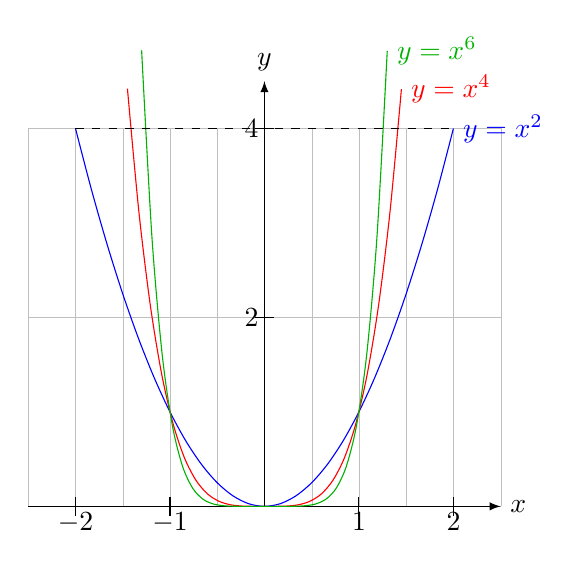
\begin{tikzpicture}[>=latex, scale=1.2]
        % Grid
        \draw[xstep=0.5,ystep=2,gray!50,ultra thin] (-2.5,0) grid (2.5,4);
        % Axes
        \draw[->] (-2.5,0) -- (2.5,0) node[right] {$x$};
        \draw[->] (0,0) -- (0,4.5) node[above] {$y$};
        % Label x and y axes
        \foreach \x in {-2,-1,1,2}
            \draw (\x,-0.1) -- (\x,0.1) node[below=2pt] {$\x$};
        \foreach \y in {2,4}
            \draw (-0.1,\y) -- (0.1,\y) node[left=2pt] {$\y$};
        % Plot y=x^2
        \draw[domain=-2:2,smooth,variable=\x,blue] plot ({\x},{\x*\x}) node[right] {$y=x^2$};
        % Plot y=x^4
        \draw[domain=-1.45:1.45,smooth,variable=\x,red] plot ({\x},{\x*\x*\x*\x}) node[right] {$y=x^4$};
        % Plot y=x^6
        \draw[domain=-1.30:1.30,smooth,variable=\x,green!70!black] plot ({\x},{\x*\x*\x*\x*\x*\x}) node[right] {$y=x^6$};
        % Dashed lines
        \draw[dashed] (-2,4) -- (2,4);
    \end{tikzpicture}

\end{document}
